\chapter{Fluorescence Anisotropy Imaging for assaying chromatin compaction states in live cells}
\begin{figure}[!htp]
    {\hfill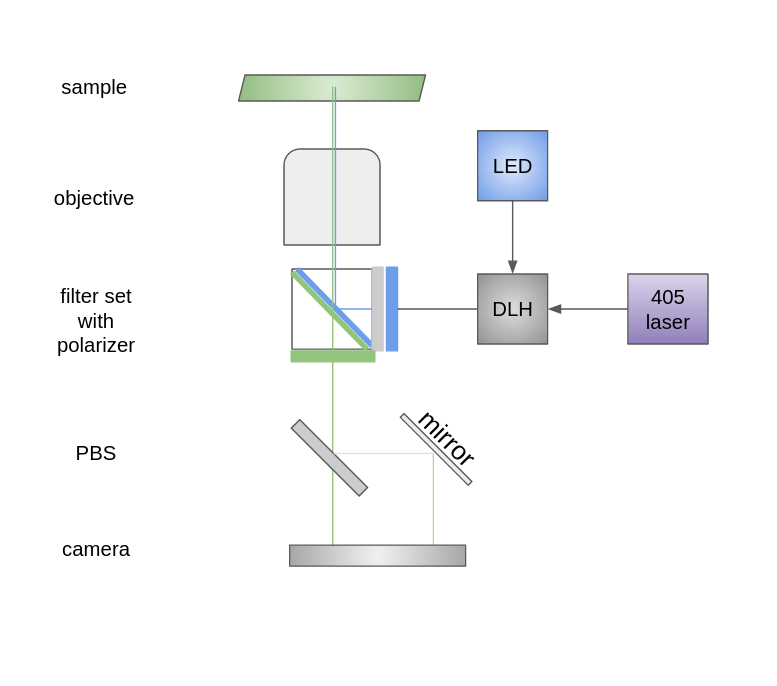
\includegraphics[trim=0 50 0 60,clip,width=0.8\linewidth]{figures/setup.png}\hspace*{\fill}}
    \caption{Fluorescence anisotropy imaging lightpath. A dual lamp housing (DLH) is used to introduce an LED light source for widefield excitation, and a 405nm laser for microirradiation, into the light path. Excitation light is polarized with a linear polarizer. Emission is collected and split with a polarizing beam splitter, which is then projected into the two halves of the camera.}
    {\label{fig:setup}}
\end{figure}
Compaction of chromatin is important in DDR, and the existing methods to study chromatin dynamics relies on fluorescently marked histones whose expansion or contraction is used as a proxy for chromatin dynamics \cite{BURGESS20141703}.  However, in experiments using microscopy, the spreading or shrinking of a chromatin region marked with a specific fluorescent histone has been used as a proxy for chromatin compaction, and as such does not report directly on physical state of the chromatin. In other studies, fluorescence anisotropy imaging (FAI) has been used to map the compaction of chromatin in living cells directly \cite{banerjee2006chromatin}. Core histone H2B tagged with EGFP is excited with polarized light, which preferentially excites EGFP molecules whose excitation dipoles are oriented along the polarization axis of the excitation light. The extent of depolarization of the emission light gives a measure of the rotational diffusion of EGFP fusion proteins. The higher the rotational diffusion, the greater is the extent of depolarization of the emission signal, over and above what would be expected because of random orientations of the fluorophores. Fluorescence anisotropy is a measure of the extent of depolarization \cite{lakowicz2013principles,ghosh2012dynamic}. Since H2B-EGFP in the regions of euchromatin should have greater rotational mobility than regions of heterochromatin, anisotropy maps generated by FAI show evidence of differential compaction of chromatin and as such could be used as a direct physical measure of local chromatin packaging \cite{bhattacharya2009spatio}. In this study, we sought to use FAI in the context of DDR to monitor chromatin compaction states directly. Chromatin decompaction is essential for repair, and yet local chromatin compaction may be used by cells to prevent further damage \cite{BURGESS20141703}. Using FAI, we studied the physical changes to the chromatin structure in response to laser microirradiation–induced clustered DSB, in regions of chromatin beyond just the site of damage. We show that anisotropy maps are preserved in fixation and regions of high and low anisotropy indeed correspond to physiologically relevant markers for heterochromatin and euchromatin, respectively. This also allows us to first follow compaction changes in response to localized DSBs in living cells, and then fix the cells and perform immunofluorescence for markers of DNA damage. Finally, we follow the differential dynamics of two endogenous damage-responsive proteins (PCNA and PARP1) with respect to chromatin compaction maps and show that their time scales of recruitment and subsequent dispersion are very different. In addition to being recruited at the site of damage, PCNA also forms nodes further away in regions of low anisotropy. These PCNA nodes in open chromatin incorporate deoxynucleotide analogs, indicating that individual DSBs from the laser-induced cluster may be extruded out from the site of damage for the purposes of repair. Together, these studies open up a new avenue of following DDR in live cells in the chromatin, while also taking advantage of different immunofluorescent markers for DNA damage and chromatin.

\section{Anisotropy Imaging}
\subsection{Microscopy}
\paragraph*{} We modified a fluorescence widefield microscope (Olympus IX83) for anisotropy imaging (Fig. \ref{fig:setup}), by introducing a polarizer in the excitation light path, and in the detection side, a polarizing beam splitter (PBS) to split the parallel and perpendicular component of light and project it in two halves of the same camera chip. This method of anisotropy imaging gives the advantage of simultaneous imaging, which would otherwise require sequential imaging or two cameras to collect the light components, with simultaneous triggers, at the cost of a smaller imaging field of view. The introduction of dual lamp housing (DLH) has the added advantage of introducing a laser in the light path of a widefield microscope, which can be used for the purpose of microirradiation, which has been used for inducing local damage on hoechst sensitized cells \cite{BURGESS20141703}. Using such a setup, we can study the physical effects on the chromatin structure with FAI, upon localized DNA damaged with microirradiation.

\subsection{Chromatin mapping}
\paragraph*{} In order to use this to map chromatin, core Histone, H2B, is tagged with EGFP and expressed in HeLa cells, which are then preferentially excited with polarized light, which maximally excites fluorophores whose excitation dipole are aligned to the polarization axis. The extent of depolarization of emission signal gives a measure of rotational diffusion of H2B-EGFP, which could be affected by its local environment. The higher the rotational diffusion, the greater is the extent of emission signal depolarizing. Anisotropy maps generated of H2B show that euchromatin like regions have greater rotational mobility than regions of heterochromatin, which is an evidence for differential packaging of chromatin compaction and can be used as a direct physical measure of chromatin packaging \cite{bhattacharya2009spatio}.

\begin{figure}[!hbtp]
    {\hfill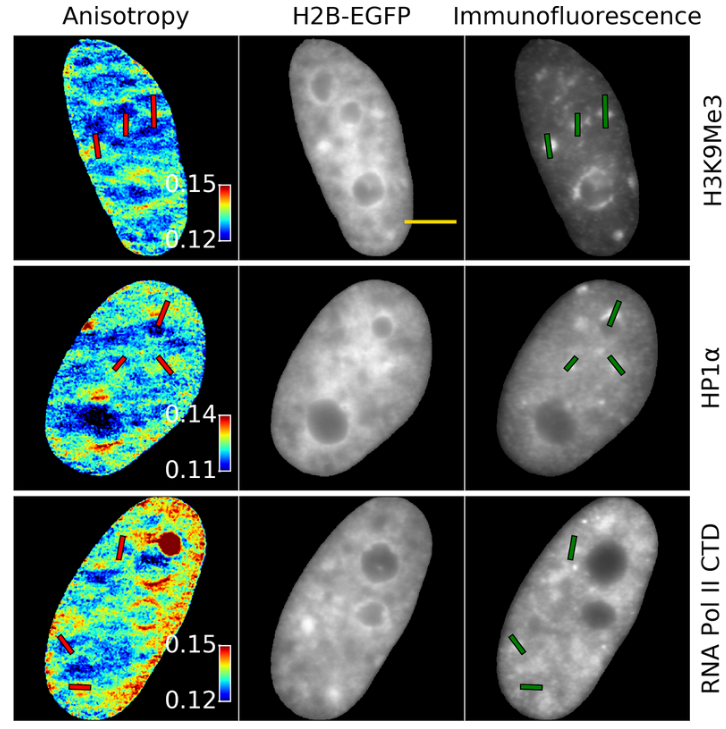
\includegraphics[trim=0 5 0 30, clip,width=0.8\linewidth]{figures/1.png}\hspace*{\fill}}
    \caption{H2B-EGFP anisotropy corresponds to known markers of heterochromatin and euchromatin. Immunofluorescence markers shown with anisotropy maps of fixed cells. HP1$\alpha$ and H3K9Me3 are known markers of heterochromatin, and phosphorylated RNA-Pol-II-CTD is a marker for active regions of transcription, where the chromatin is more open. Scale bar corresponds to 5$\mu$m.}
    {\label{fig:an_verify}}
\end{figure}

\begin{figure}[!hbtp]
    {\hfill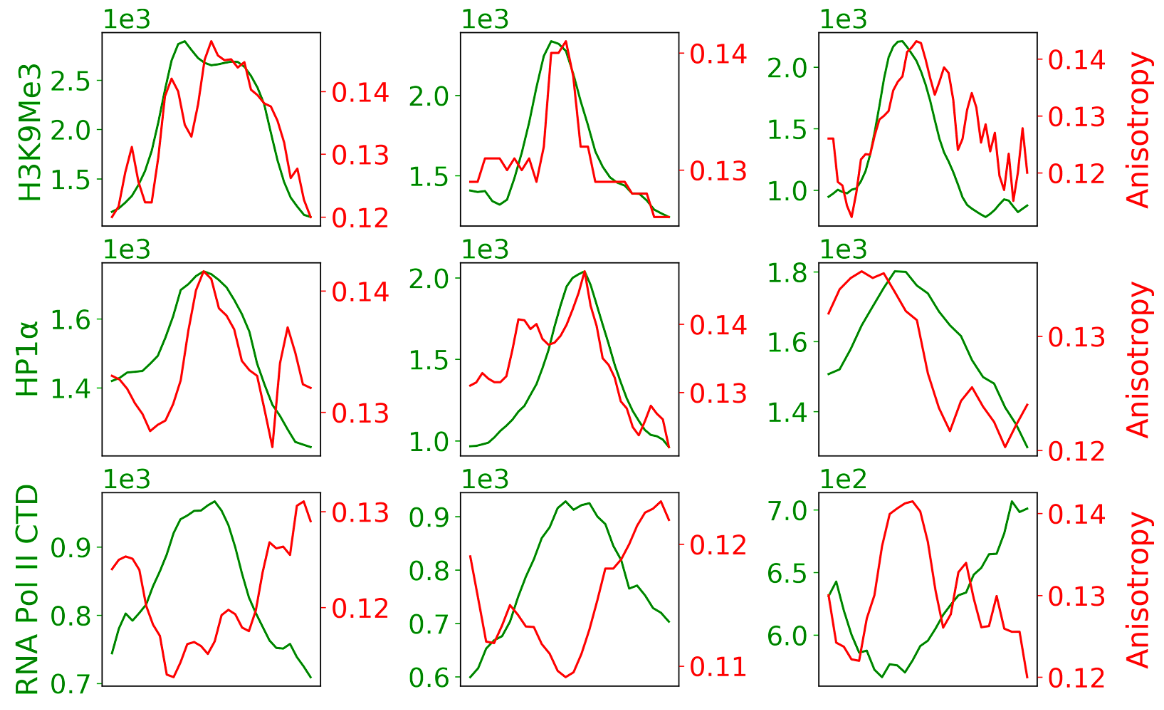
\includegraphics[clip,width=0.8\linewidth]{figures/2.png}\hspace*{\fill}}
    \caption{H2B-EGFP anisotropy corresponds to known markers of heterochromatin and euchromatin. Line profile of lines draw in the images in (Fig. \ref{fig:an_verify}) (green in immunofluorescence image, red in anisotropy map). Line profiles show that heterochromatin corresponds to regions of high anisotropy, while euchromatin corresponds to regions of low anisotropy. X-axis is distance along the line.}
    {\label{fig:an_verify_line}}
\end{figure}


\paragraph*{} In order to verify that the anisotropy values indeed correspond to biologically relevant structures of chromatin, we first demonstrated that anisotropy maps are preserved in fixation; we then imaged HeLa cells expressing H2B-EGFP for known markers of chromatin structures with immunofluorescence assay. We found that trimethylated lysine at ninth position in core Histone H3 (H3K9Me3), which is generally associated with densely packed heterochromatin regions correspond to high values of anisotropy (Fig. \ref{fig:an_verify}, \ref{fig:an_verify_line}). Similarly, we found that Heterochromatin Protein 1$\alpha$ (HP1$\alpha$), associated with heterochromatin domains, are also enriched in regions of high anisotropy. Conversely, we stained for decompacted chromatin using an antibody against the activated form of RNA polymerase, in which S5 is phosphorylated in C-terminal domain, and found that the anisotropy values are low in such regions. Together, these results suggested that regions of high and low anisotropy indeed correspond to biologically relevant structures of dense and loosely packed chromatin.  

\begin{figure}[H]
    {\hfill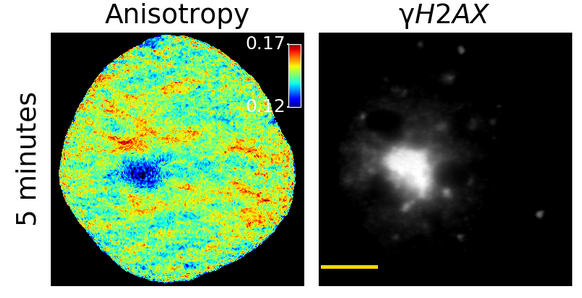
\includegraphics[clip,width=0.8\linewidth]{figures/micro_gh2ax.png}\hspace*{\fill}}
    \caption{Microirradiation activates DNA damage responses. $\gamma$H2AX, a known marker for damage response, is found at the site of microirradiation.}
    {\label{fig:micro_gh2ax}}
\end{figure}
\paragraph*{} We verified that microirradiation indeed causes damage by fixing and staining microirradiated cells for $\gamma$H2AX, which was observed at the site of damage (Fig. {\ref{fig:micro_gh2ax}}), indicating activated damage response.




The main strength of FAI is that it can report on chromatin compaction states in living cells. And because anisotropy maps are preserved in fixation, as demonstrated in the previous section, live-cell dynamics upon DNA damage can be followed by immunofluorescent detection of damage markers in the very same cells. We used FAI to study the changes to chromatin structure that has undergone microirradiation induced DSBs as employed by previous studies (Kruhlak et al., 2006; Burgess et al., 2014; Strickfaden et al., 2016). We modified our FAI microscope to introduce a 405-nm laser into the light path and used Hoechst-sensitized cells to cause local double-strand breaks of the DNA. Minutes after irradiation, strong staining for $\Gamma$H2AX and the phosphorylated form of Chk1 (p-Chk1, a target of the master DDR kinase ATR) was observed at the site of damage (Supplemental Figure 4), which indicated that the damage response was in action. Using this microirradiation protocol, we collected anisotropy data for the damaged cells over a period of 2 h, imaged once every 5 min. Anisotropy at the site of the damage could not be ascertained due to localized photobleaching of H2B-EGFP upon irradiation, but the response of the rest of the chromatin, which did not see direct irradiation, could be followed. In comparison to the control undamaged cells (N = 13), the overall $\Delta$anisotropy value ($\Delta$anisotropy = rt – r0, where rt is the mean anisotropy at any given time point, and r0 is the mean anisotropy for the 0th time point) of the irradiated cells increased with time (Figure 2B), though the response was heterogeneous among cells (Supplemental Figure 5). And though the mean rise is small, one should keep in mind that anisotropy values are themselves fractional; also, mean anisotropy averages over regions where compaction increases and surrounding regions where it decreases correspondingly, keeping the changes in mean anisotropy small. This heterogeneity is captured in the anisotropy maps, and indeed a fraction of cells show formation of nodes of high local compaction even in regions that have not directly been damaged (Figure 2A). To quantify this better and visualize the nodes, we thresholded the anisotropy map with a threshold value of “mean + 2 sigma,” where mean is the mean anisotropy value of the nucleus before damage and sigma is the SD. Values below the threshold are turned to gray, so that it becomes easier to visualize the high–anisotropy value pixels formed upon irradiation (Supplemental Figure 5C). The formation of high-anisotropy nodes is reflected in the overall increase in high-anisotropy pixels for irradiated cells as compared with control cells. However, it should be noted that the control cells also show a fair degree of heterogeneity among themselves, and this could be because of toxic effects of the imaging excitation light (Ge et al., 2013), natural cell cycle–driven processes that causes chromatin compaction changes, or systematic changes to anisotropy with photobleaching. Nonetheless, the propensity for increased compaction in irradiated cells is clear and significantly different from the dynamics of control cells. When the individual $\Delta$anisotropy time trace for each irradiated cell is examined closely (Supplemental Figure 5), 21 out of 27 cells show positive increase in delta anisotropy and only 6 out of 27 cells show an overall negative trend over the 2 h after damage, whereas in control cells, 7 out of 13 cells show a positive trend and 6 out of 13 cells show a negative trend. This indicates that there is inherent variability in the cellular response to damage, but overall there is condensation of chromatin in response to damage.

Next we wanted to combine the time course of anisotropy imaging with live-cell detection of other markers of the damage response. For this, we chose chromobody-mediated detection of early and late markers of DDR—PARP1 and PCNA. PARP1 is known to be transiently enhanced at sites of damage in response to irradiation-induced DSBs (Chou et al., 2010; Qi et al., 2019), while PCNA, being the DNA clamp, would be required for the processivity of the DNA polymerase in the final steps of repair (Moldovan et al., 2007). We independently transfected PARP1 and PCNA chromobodies tagged with TagRFP in HeLa cells stably expressing H2B-EGFP. Chromobodies (ChromoTek) are small intracellular antibodies tagged with fluorescent protein. Their major advantage is that they detect the endogenous proteins they are designed against without artifacts of overexpression of those proteins in transient transfections (Burgess et al., 2012; Panza et al., 2015). As expected, PARP1 was recruited to the site of damage almost immediately upon irradiation (Figure 3A). However, the PARP1 signal diffused away from the site by 15 min after damage, as expected (Haince et al., 2008; Mortusewicz et al., 2007). To our surprise, however, PCNA, which should be involved in the repair only at later stages, was also recruited immediately to the site of damage (Figure 3B). This was the case in G1 and G2 cells where the PCNA chromobody was homogenous in the nucleus, and even in S phase cells where the PCNA chromobody was punctated, as PCNA follows the replication fork (Supplemental Movies 1 and 2). The PCNA chromobody is primarily used for cell-cycle stage detection (Burgess et al., 2012). This implies that in response to clustered DSBs, even PCNA from replication forks is recruited to the site of damage. PCNA persisted at the site of damage for the duration of the time course, longer than PARP1 (Figure 3C). This local enrichment was quantified by plotting the mean intensity of the chromobody at the site of damage normalized to the mean intensity outside. (We found this to be a more robust metric for the enrichment, compared with just the normalized intensity at the site of damage, which decays due to photobleaching during the time course, in addition to actual dynamics. This metric is more robust because photobleaching operates both within and outside the site of damage.) But while PCNA persists longer, within 20 min, there are nodes of PCNA formed, away from the site of damage, which correspond to regions of lower anisotropy (Figure 3; Supplemental Figure 6). We asked whether these sites of PCNA enrichment and low anisotropy represent simply sites of repair factor storage or of active repair. We reasoned that if they are indeed sites of repair, even in the G1 or G2 phase, we may be able to see incorporation of a deoxynucleotide analog such as ethynyl deoxyuridine (EdU). HeLa cells transfected with the PCNA chromobody were subjected to laser-induced DSBs. G1 or G2 cells that have a homogenous distribution of the PCNA chromobody in the nucleus were chosen. We observed that at these sites of transient PCNA nodes, EdU is incorporated, which is an indication of new DNA being synthesized at these sites (Figure 3E; Supplemental Figure 7). We ruled out bleedthrough of PCNA signal in the EdU channel by imaging plates for cells with and without EdU treatment (Supplemental Figure 7). Thus, though the DSBs are induced locally, these nodes of PCNA incorporating EdU further away may indicate a looping out of individual DSBs from the site of primary damage.


Steady-state fluorescence anisotropy imaging has been used previously for measuring chromatin compaction in living cells (Banerjee et al., 2006). We established that anisotropy maps are preserved in fixation, and regions of high and low anisotropy indeed correspond to heterochromatin and euchromatin, respectively. In the context of DDR, our fluorescence anisotropy imaging studies suggest that the undamaged chromatin is globally compacted in response to localized DSB damage. In regions away from the site of damage, we observe chromatin nodes forming, as well as transient accumulation of phospho-ATM and PCNA in specific sites that correspond to more loosely packed regions of chromatin. These low-anisotropy regions with accumulated repair proteins could be regions of repair or of factors poised for repair. In future studies, we aim to investigate the possibility of blocking damage response in cells using small molecule inhibitors for DDR master kinases and what effects it has on the chromatin response upon damage. A limitation of this study is that we follow the response of undamaged chromatin because of local clustered DSBs, but anisotropy information is lost at the site of damage because of photobleaching. This could potentially be circumvented by using a histone H2B tagged with photoactivable GFP (H2B-PA-GFP). Condensation of the damaged chromatin could indeed be observed in such an experiment (Supplemental Figure 8).



\paragraph*{} In summary, we developed fluorescence anisotropy imaging to map regions of chromatin in live cells, and incorporated microirradiation to damage chromatin, and measure its dynamics post damage with live cell imaging. Following live cell imaging, we fixed the cells, and performed immunofluorescence assay against known markers of damage response to observe the state of those endogenous proteins.
